\documentclass[epsfig,10pt,fullpage]{article}

\newcommand{\LabNum}{11}
\newcommand{\CommonDocsPath}{../../../common/docs}
\addtolength{\textwidth}{1.5in}
\addtolength{\oddsidemargin}{-0.75in}
\addtolength{\topmargin}{-0.75in}
\addtolength{\textheight}{1.5in}
\addtolength{\evensidemargin}{0.75in}
\setlength\parindent{0pt}
\raggedbottom

\usepackage{ae,aecompl}
\usepackage{epsfig,float,times}
\usepackage[hypcap]{caption}
\usepackage[pdftex, colorlinks]{hyperref}
\usepackage{graphicx}
\usepackage[usenames, dvipsnames]{color}
\usepackage{rotating}
\usepackage{tikz}
\usetikzlibrary{automata,positioning}
\usepackage{placeins}

\widowpenalty 10000
\clubpenalty 10000

\newcommand{\red}[1]{{\color{red}\sf{#1}}}
\newcommand{\green}[1]{{\color{green}\sf{#1}}}
\newcommand{\blue}[1]{{\color{blue}\sf{#1}}}
\definecolor{PineGreen}{rgb}{0.0, 0.47, 0.44}
\definecolor{ForestGreen}{rgb}{0.13, 0.55, 0.13}
\definecolor{Brown}{rgb}{0.59, 0.29, 0.0}

\newcommand{\UPDatePublished}{Oct 2021}
\newcommand{\versnum}{21.1} %version number quartus/AMP
\newcommand{\quartusname}{Quartus\textsuperscript{\textregistered} Prime}	
\newcommand{\UPTextBar}{For \quartusname{} \versnum{}}
\newcommand{\thisyear}{2021 } %for copyright
\newcommand{\company}{FPGAcademy.org}
\newcommand{\longteamname}{FPGAcademy.org}
\newcommand{\teamname}{FPGAcademy}
\newcommand{\website}{FPGAcademy.org}

\newcommand{\productAcronym}{AMP}
\newcommand{\productNameShort}{Monitor Program}

\newcommand{\productNameMedTM}{A Monitor Program}
\newcommand{\productNameMed}{A Monitor Program}

%\newcommand{\headerLogoFilePath}[1]{#1/FPGAcademy.png}

% listings is a package that supports encapsulating source code in LaTeX conveniently
\usepackage{listings}

\def\expandparam\lstinputlisting[#1]#2{\edef\tmp{\noexpand\lstinputlisting[#1]{#2}}\tmp}

%%%%%%%%%%%%%%%%%%%% Source Code Formatting %%%%%%%%%%%%%%%%%%%%
\definecolor{globalCommentColour}{rgb}{0.588,0.588,0.588}

%%%%%%%%%%%%%%%%%%%%%%%%%%%%%%%%%%%%%%%%%%%%%%%%%%%%
% Defining language style
% NiosII ASM
\lstdefinelanguage[NiosII]{Assembler} {
  morekeywords={add, addi, and, andhi, andi, beq, bge, bgeu, bgt, bgtu, ble,  bleu, blt, bltu, bne, br, break,
  bret, call, callr, cmpeq, cmpeqi, cmpge, cmpgei, cmpgeu, cmpgeui, cmpgt, cmpgti, cmpgtu, cmpgtui, cmple,
  cmplei, cmpleu, cmpleui, cmplt, cmplti, cmpltu, cmpltui, cmpne, cmpnei, custom, div, divu, eret, flushd,
  flushda, flushi, flushp, initd, initda, initi, jmp, jmpi, ldb, ldbio, ldbu, ldbuio, ldh, ldhio, ldhu, ldhuio,
  ldw, ldwio, mov, movhi, movi, movia, movui, mul, muli, mulxss, mulxsu, mulxuu, nextpc, nop, nor, or, orhi, ori,
  rdctl, rdprs, ret, rol, roli, ror, sll, slli, sra, srai, srl, srli, stb, stbio, sth, sthio, stw, stwio,
  sub, subi, sync, trap, wrctl, wrtcl, wrprs, xor, xori, xorhi, xori},
  morekeywords=[2]{.abort, .ABORT, .align, .app-file, .ascii, .asciz, .balign, .byte, .comm, .data, .def,
  .desc, .dim, .double, .eject, .else, .end, .endef, .endif, .equ, .equiv, .err, .extern, .file, .fill, .float,
  .global, .globl, .hword, .ident, .if, .include, .int, .irp, .irpc, .lcomm, .lflags, .line, .linkonce, .ln,
  .list, .long, .macro, .mri, .nolist, .octa, .org, .p2align, .psize, .quad, .rept, .sbttl, .scl, .section,
  .set, .short, .single, .size, .sleb128, .skip, .space, .stadb, .stabn, .stabs, .string, .symver, .tag,
  .text, .title, .type, .val, .uleb128, .word},
  morekeywords=[3]{et, bt, gp, sp, fp, ea, sstatus, ra, pc, status, estatus, bstatus, ienable, ipending, cpuid,
  exception, pteaddr, tlbacc, tlbmisc, eccinj, badaddr, config, mpubase, mpuacc},
  sensitive=t,
  alsoletter=.,
  morestring=[b]",
  morecomment=[s]{/*}{*/},
  morecomment=[l]\#,
}[keywords,comments,strings]
   
%% NOTE: morekeywords=[2] are GNU directives.
   
\definecolor{niosInstructionColour}{rgb}{0.000,0.608,0.000}
\definecolor{niosDirectiveColour}{rgb}{0.000,0.000,0.902}
\definecolor{niosSpecialRegColour}{rgb}{0.000,0.000,0.000}
\definecolor{niosStringColour}{rgb}{0.808,0.482,0.000}
   
%% NOTE: To make bold use: =\bfseries\color{<colour>}
\lstdefinestyle{defaultNiosStyle} {
  language=[NiosII]{Assembler},
  stringstyle=\color{niosStringColour},
  keywordstyle=\color{niosInstructionColour},
  keywordstyle=[2]\color{niosDirectiveColour},
  keywordstyle=[3]\itshape\color{niosSpecialRegColour}
}
%%%%%%%%%%%%%%%%%%%%%%%%%%%%%%%%%%%%%%%%%%%%%%%%%%%%

%%%%%%%%%%%%%%%%%%%%%%%%%%%%%%%%%%%%%%%%%%%%%%%%%%%%
% Defining language style
% ArmA9 ASM
\lstdefinelanguage[ArmA9]{Assembler} {
  morekeywords={ADC, ADD, ADDS, AND, ANDS, B, BAL, BEQ, BGE, BGT, BL, BLT, BIC, BKPT, BLX, BNE, BX, CDP, CLZ, CMN, CMP, EOR,
  EORS, LDC, LDM, LDR, LDRB, LDRBT, LDRH, LDRSB, LDRSH, LDRT, LSL, MCR, MLA, MOV, MOVW, MOVT, MRC, MRS, MSR, MUL, MVN, ORR, PLD,
  ROR, RSB, RSC, SBC, SMLAL, SMULL, STC, STM, STR, STRB, STRBT, STRH, STRT, SUB, SUBS, SWI, SWP, SWPB, TEQ, UMLAL,
  PUSH, POP, MOVS, RORS, LSR},
  morekeywords=[2]{.abort, .ABORT, .align, .app-file, .ascii, .asciz, .balign, .byte, .comm, .data, .def,
  .desc, .dim, .double, .eject, .else, .end, .endef, .endif, .equ, .equiv, .err, .extern, .file, .fill, .float,
  .global, .globl, .hword, .ident, .if, .include, .int, .irp, .irpc, .lcomm, .lflags, .line, .linkonce, .ln,
  .list, .long, .macro, .mri, .nolist, .octa, .org, .p2align, .psize, .quad, .rept, .sbttl, .scl, .section,
  .set, .short, .single, .size, .sleb128, .skip, .space, .stadb, .stabn, .stabs, .string, .symver, .tag,
  .text, .title, .type, .val, .vectors, .uleb128, .word},
  morekeywords=[3]{SP, PC, MIDR, CTR, TCMTR, TLBTR, MPIDR, ID_PFR0, ID_PFR1, ID_DFR0, ID_MMFR0, ID_MMFR1, ID_MMFR2,
  ID_MMFR3, ID_ISAR0, ID_ISAR1, ID_ISAR2, ID_ISAR3, ID_ISAR4, CCSIDR, CLIDR, AIDR, CSSELR, TTBR0, TTRB1, TTBR2, DACR,
  DFSR, IFSR, ADFSR, AIFSR, DFAAR, IFAR, ICIALLUIS, BPIALLIS, PAR, ICIALLU, ICIMVAU, BPIALL, DCIMVAC, DCISW, V2PCWPR,
  DCCVAC, DCCSW, DDIMVAC, DCISW, TLBALLIS, TLBIMVAIS, TLBIASIDIS, TLBIMVAAIS, TLBIALL, TLBIMVA, TLBIASID, TLBIMVAA,
  PMCR, PMCNTENSET, PMCNTENCLR, PMOVSR, PMSWINC, PMSELR, PMXEVTYPER, PMXEVCNTR, PMUSERENR, PMINTENSET, PMINTENCLR,
  PRRR, NRRR, PLEIDR, PLEASR, PLEFSR, PLEUAR, PLEPCR, VBAR, MVBAR, ISR, FCSEIDR, CONTEXTIDR, TPIDRURW, TPIDRURO, TPIDRPRW},
  sensitive=f,
  alsoletter=.,
  morestring=[b]",
  morecomment=[s]{/*}{*/},
  morecomment=[l]{//},
}[keywords,comments,strings]
   
%% NOTE: morekeywords=[2] are GNU directives.
   
\definecolor{armInstructionColour}{rgb}{0.000,0.608,0.000}
\definecolor{armDirectiveColour}{rgb}{0.000,0.000,0.902}
\definecolor{armSpecialRegColour}{rgb}{0.000,0.000,0.000}
\definecolor{armStringColour}{rgb}{0.808,0.482,0.000}
   
\lstdefinestyle{defaultArmStyle} {
  language=[ArmA9]{Assembler},
  stringstyle=\color{armStringColour},
  keywordstyle=\color{armInstructionColour},
  keywordstyle=[2]\color{armDirectiveColour},
  keywordstyle=[3]\itshape\color{armSpecialRegColour}
}
%%%%%%%%%%%%%%%%%%%%%%%%%%%%%%%%%%%%%%%%%%%%%%%%%%%%

%%%%%%%%%%%%%%%%%%%%%%%%%%%%%%%%%%%%%%%%%%%%%%%%%%%%
% Defining language style
% FPGAcademy ASM
\lstdefinelanguage{ASM}{
  morekeywords = [1]{mv, mvt, mvne, mvcc, add, sub, st, ld, and, b, bne, beq, bcc, bcs},
  morekeywords = [2]{word, define},
  keywordstyle = [1]\color{ForestGreen},
  keywordstyle = [2]\color{blue},
  sensitive = true,
  morecomment = [l]{//},
}

\lstset{
  language = ASM,
  basicstyle=\small\color{black}\ttfamily,
  commentstyle=\small\color{Brown}\itshape\ttfamily,
  showstringspaces=false,
  frame=none, %lines % boxed listings
  breaklines=true,
  breakatwhitespace=true,
  tabsize=3
}
%%%%%%%%%%%%%%%%%%%%%%%%%%%%%%%%%%%%%%%%%%%%%%%%%%%%

%%%%%%%%%%%%%%%%%%%%%%%%%%%%%%%%%%%%%%%%%%%%%%%%%%%%
% Defining language style
% Java
\definecolor{javaStringColour}{rgb}{0.808,0.482,0}
%%%%%%%%%%%%%%%%%%%%%%%%%%%%%%%%%%%%%%%%%%%%%%%%%%%%

%%%%%%%%%%%%%%%%%%%%%%%%%%%%%%%%%%%%%%%%%%%%%%%%%%%%
% Defining language style
% C
\definecolor{CStringColour}{rgb}{0.808,0.482,0}

\lstset{
  language = C,
  basicstyle=\small\color{black}\ttfamily, 
  commentstyle=\small\color{PineGreen}\itshape\ttfamily,
  keywordstyle=\small\color{blue}\bfseries\ttfamily,
  showstringspaces=false,
  frame=none, %lines % boxed listings
  breaklines=true,
  breakatwhitespace=true,
  tabsize=3
}
%%%%%%%%%%%%%%%%%%%%%%%%%%%%%%%%%%%%%%%%%%%%%%%%%%%%

%%%%%%%%%%%%%%%%%%%%%%%%%%%%%%%%%%%%%%%%%%%%%%%%%%%%
% Defining language style
% Verilog
\definecolor{verilogCommentColour}{rgb}{0.000,0.502,0.000}

\lstdefinestyle{defaultVerilogStyle} {
  language={Verilog},
  keywordstyle=\color{blue},
  commentstyle=\color{verilogCommentColour}
}
%%%%%%%%%%%%%%%%%%%%%%%%%%%%%%%%%%%%%%%%%%%%%%%%%%%%

%%%%%%%%%%%%%%%%%%%%%%%%%%%%%%%%%%%%%%%%%%%%%%%%%%%%
% Defining language style
% VHDL
\lstdefinestyle{defaultVHDLStyle} {
  language={VHDL},
  keywordstyle=\color{blue},
  commentstyle=\color{verilogCommentColour}
}
%%%%%%%%%%%%%%%%%%%%%%%%%%%%%%%%%%%%%%%%%%%%%%%%%%%%

%%%%%%%%%%%%%%%%%%%%%%%%%%%%%%%%%%%%%%%%%%%%%%%%%%%%
% Defining language style
% LaTeX
\lstdefinelanguage[LocalLaTeX]{TeX}[LaTeX]{TeX}{moretexcs={bf, it, sf, lstset},}

\lstdefinestyle{defaultLocalLatexStyle} {
  language=[LocalLatex]{TeX},
  keywordstyle=\color{blue}\bfseries,
  keywordstyle=[2]\color{blue},
  keywordstyle=[3]\color{blue}\bfseries
}
%%%%%%%%%%%%%%%%%%%%%%%%%%%%%%%%%%%%%%%%%%%%%%%%%%%%

%%%%%%%%%%%%%%%%%%%%%%%%%%%%%%%%%%%%%%%%%%%%%%%%%%%%
% Defining language style
% Default
\lstset{
  basicstyle=\small\color{black}\ttfamily,
  commentstyle=\small\color{globalCommentColour}\itshape\ttfamily,
  keywordstyle=\small\color{blue}\bfseries\ttfamily,
  showstringspaces=false,
  frame=none, %lines % boxed listings
  breaklines=true,
  breakatwhitespace=true,
  tabsize=3
}
%%%%%%%%%%%%%%%%%%%%%%%%%%%%%%%%%%%%%%%%%%%%%%%%%%%%


\hypersetup{
  pdftitle={Digital Logic Lab Exercise \LabNum},
  linkcolor=blue,
  hyperindex=true,
  pdfauthor={FPGAcademy.org},
  pdfkeywords={FPGAcademy.org, FPGAcademy, Lab, Exercise, Digital Logic},
  bookmarks,
  bookmarksopen=false,
  filecolor=blue,
  pdfstartview={FitH},
  urlcolor=blue,
  plainpages=false,
  pdfpagelabels=true,
  linkbordercolor={1 1 1} %no color for link border
}



\begin{document}

\centerline{\huge Digital Logic}
~\\
\centerline{\huge Laboratory Exercise \LabNum}
~\\
\centerline{\large Implementing Algorithms in Hardware}
~\\

This is an exercise in using algorithmic state machine charts to implement algorithms as hardware circuits.

\section*{Background}
\addcontentsline{toc}{1}{Background}
Algorithmic State Machine (ASM) charts are a design tool that allow
the specification of digital systems in a form similar to a flow chart. An example of
an ASM chart is shown in Figure~\ref{fig:bit_counting_asm}. It represents a circuit that 
counts the number of bits set to 1 in an n-bit input A ($A=a_{n-1}a_{n-2}{\ldots}a_1a_0$).
The rectangular boxes in this diagram represent the {\it states} of the digital system, 
and actions specified inside of a state box occur on each active clock edge in this
state.  Transitions between states are specified by arrows. 
The diamonds in the ASM chart represent conditional tests, and the ovals represent 
actions taken only if the corresponding conditions are either true (on an arrow labeled 1) 
or false (on an arrow labeled 0).

\begin{figure}[H]
\begin{center}
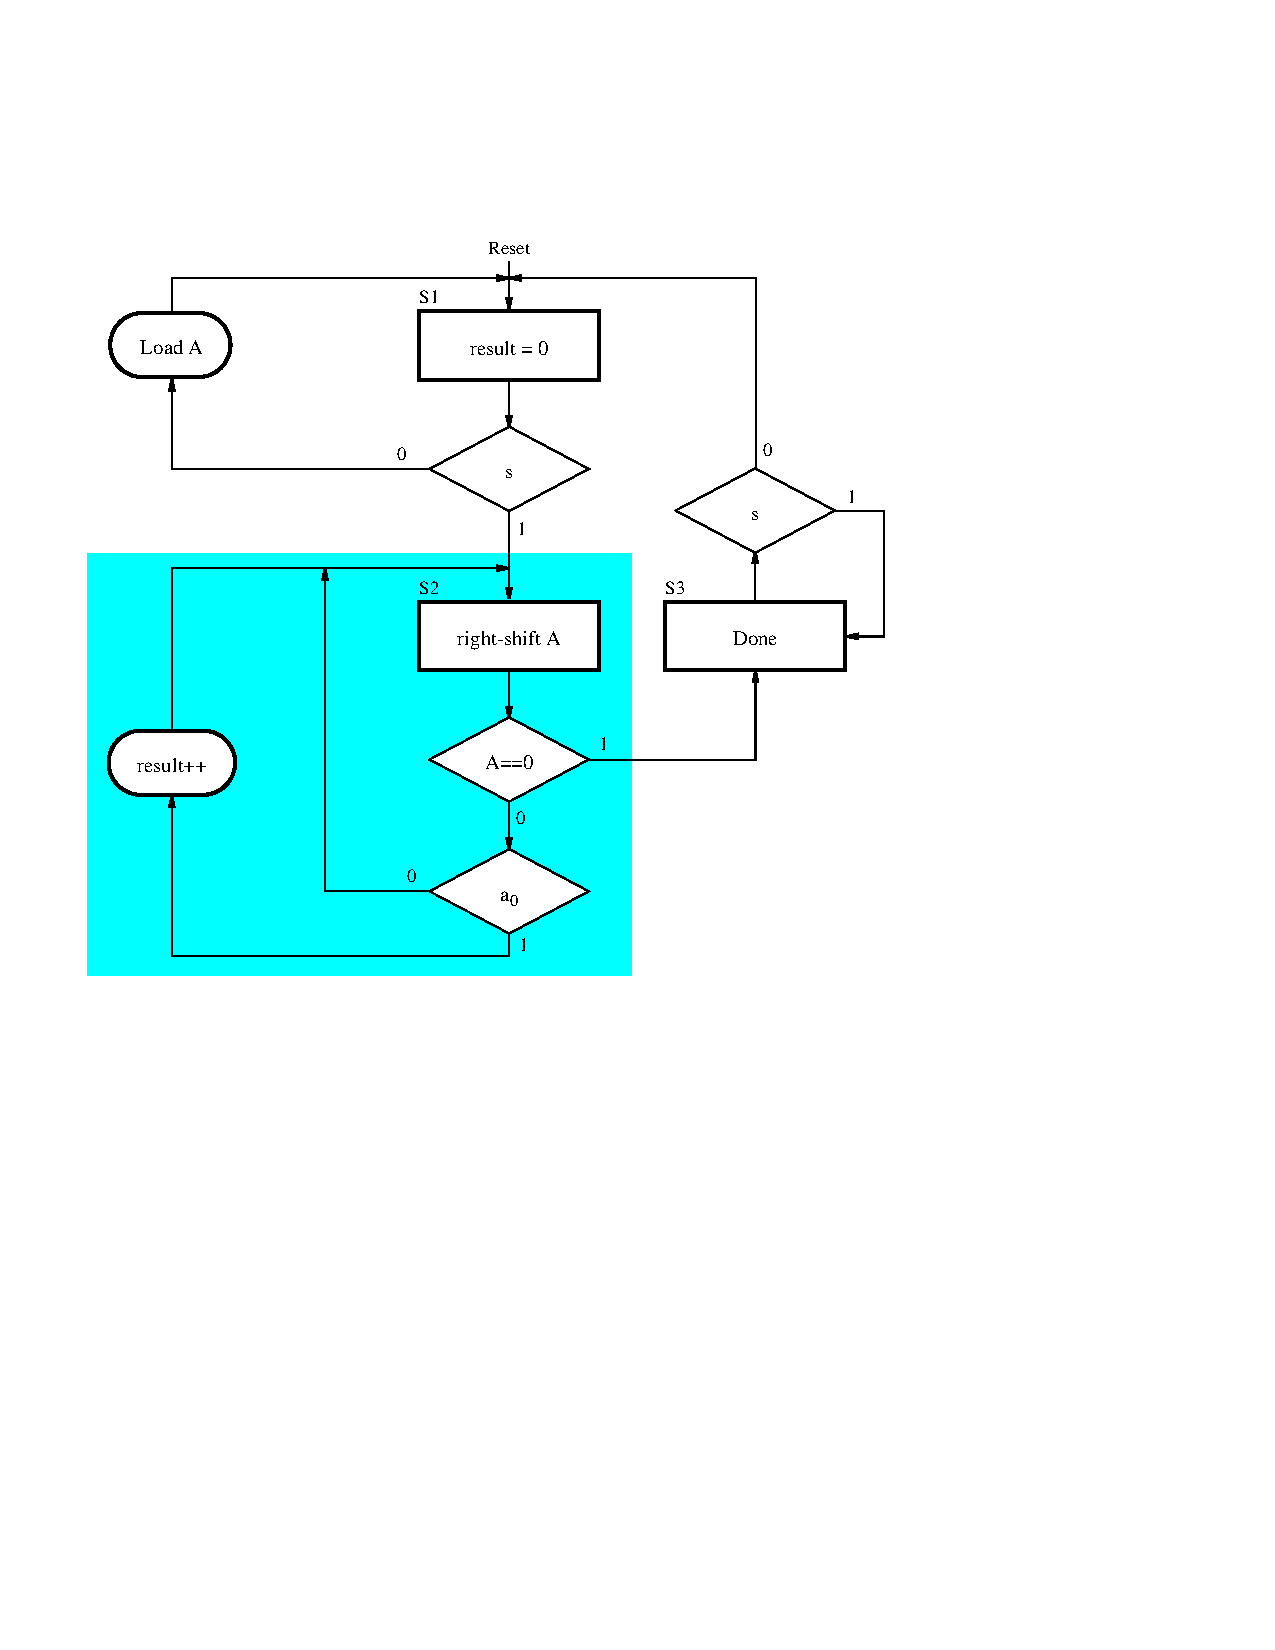
\includegraphics{figures/bit_counting_asm}
\end{center}
\caption{ASM chart for a bit counting circuit.}
\label{fig:bit_counting_asm}
\end{figure}

In this ASM chart, state $S1$ is the initial state. In this state the {\it result} is
initialized to 0, and data is loaded into a register {\it A}, until a start signal,
{\it s}, is asserted.  The ASM chart then transitions to state $S2$, where it increments
the {\it result} to count the number of 1's in register {\it A}. Since state $S2$
specifies a shifting operation, then $A$ should be implemented as a shift register. 
Also, since the {\it result} is incremented, then this variable should be implemented as a
counter.  When register $A$ contains 0 the ASM chart transitions to state $S3$, where it sets an 
output {\it Done} $=1$ and waits for the signal $s$ to be deasserted.

~\\
A key distinction between ASM charts and flow charts is a concept known as {\it implied timing}. 
The implied timing specifies that all actions associated with a given state take place
only when the system is in that state when an active clock edge occurs. For example, when
the system is in state $S1$ and the start signal $s$ becomes 1, then the next active clock
edge performs the following actions: initializes {\it result} to 0, and transitions to 
state $S2$. The action {\it right-shift A} does not happen yet, because the system is not yet 
in state $S2$. For each active clock cycle in state $S2$, the actions highlighted in 
Figure~\ref{fig:bit_counting_asm} take place, as follows: increment {\it result} if bit
$a_0 = 1$, change to state~$S3$ if $A = 0$ (or else remain in state $S2$), and shift $A$ to
the right. 

~\\
The implementation of the bit counting circuit includes the counter to store the {\it result} and
the shift register $A$, as well as a finite state machine.  The FSM is often referred to as 
the {\it control} circuit, and the other components as the {\it datapath} circuit. 

\section*{Part I}
\addcontentsline{toc}{2}{Part I}
Write VHDL code to implement the bit-counting circuit using the ASM chart shown in
Figure~\ref{fig:bit_counting_asm} on a DE-series board. Include in your VHDL code the
datapath components needed, and make an FSM for the control circuit. The inputs to your 
circuit should consist of an 8-bit input connected to slide switches {\it SW}$_{7-0}$, a
synchronous reset connected to {\it KEY}$_0$, and a start signal
({\it s}) connected to switch {\it SW}$_9$. Use the 50 MHz clock signal provided on the
board as the clock input for your circuit. Be sure to synchronize the $s$ signal to the 
clock. Display the number of~1s counted in the input data on the 7-segment display HEX0, and 
signal that the algorithm is finished by lighting up {\it LEDR}$_9$.

\section*{Part II}
\addcontentsline{toc}{3}{Part II}
We wish to implement a binary search algorithm, which searches through an array to locate 
an 8-bit value {\it A} specified via switches {\it SW}$_{7-0}$. A block diagram for the 
circuit is shown in Figure~\ref{fig:binary_search_cct}.

\begin{figure}[H]
	\begin{center}
		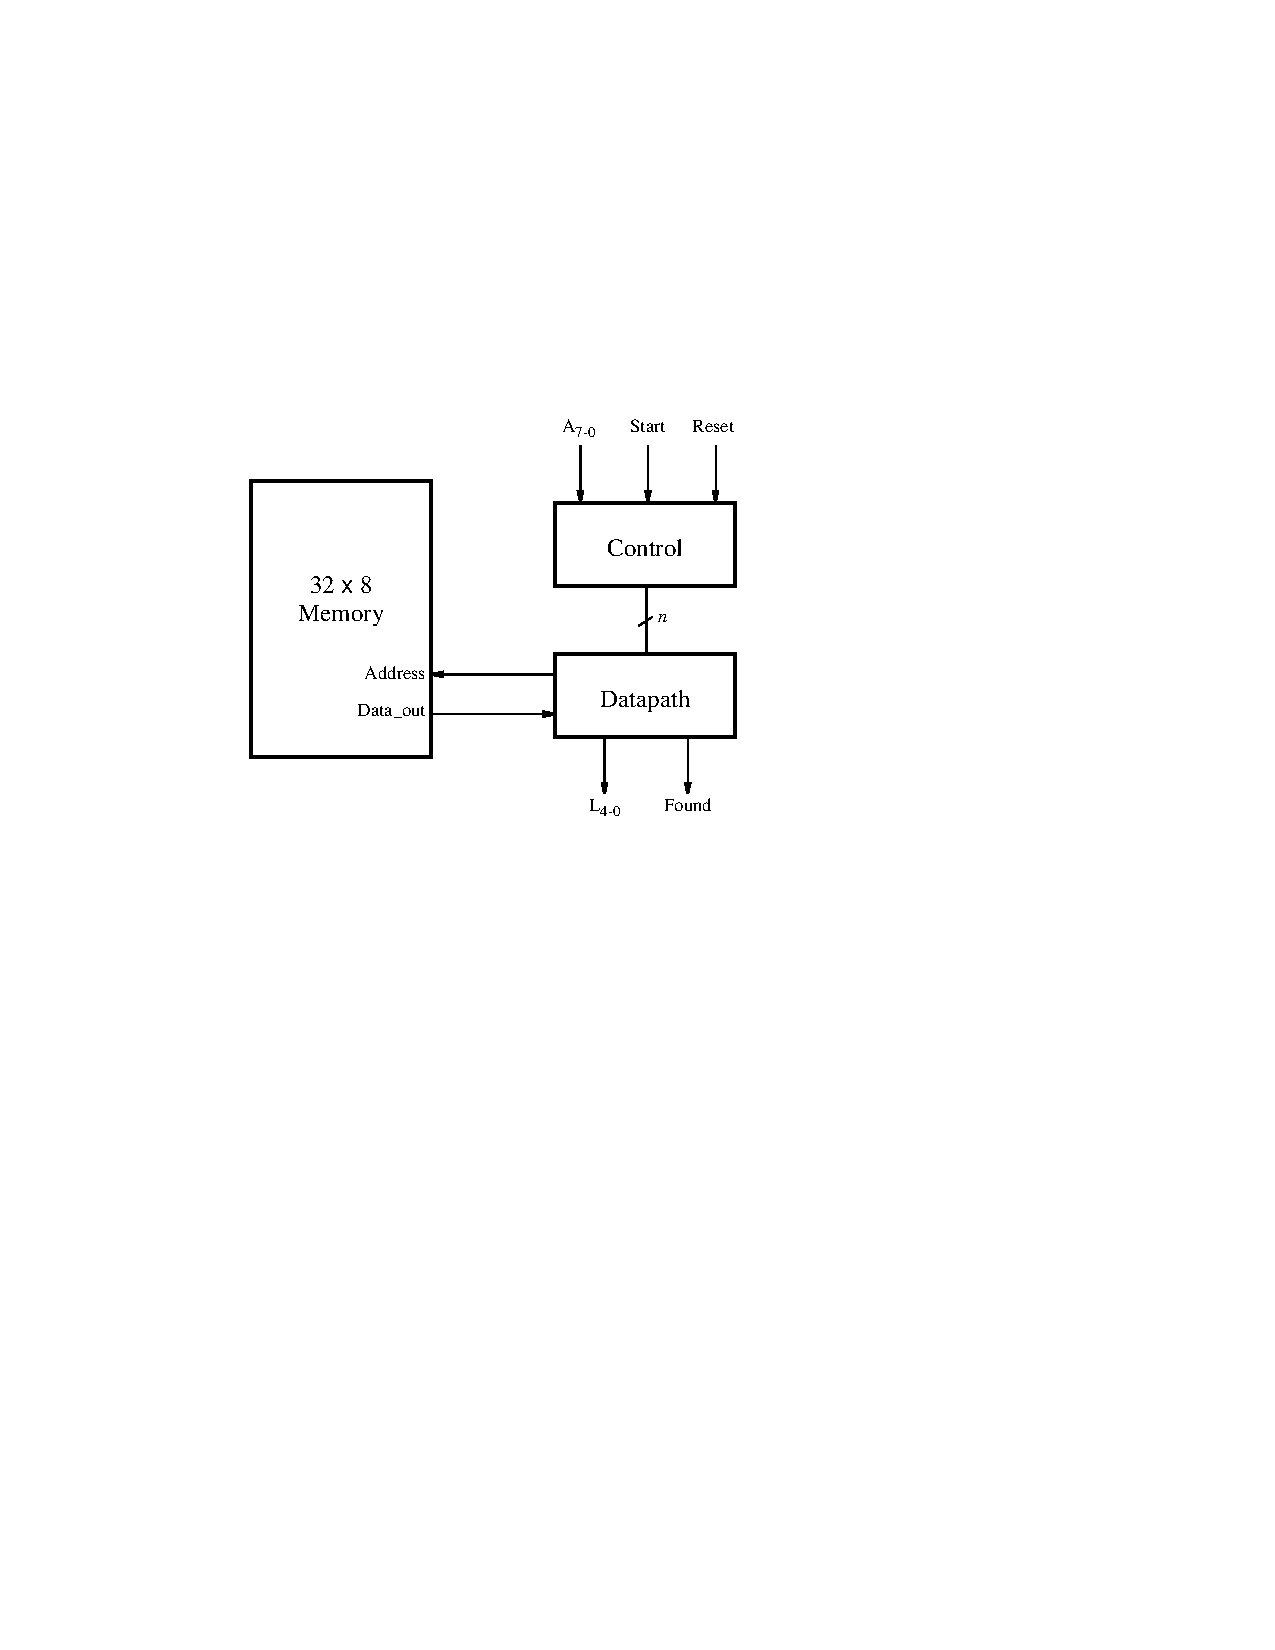
\includegraphics[]{figures/binary_search_circuit.pdf}
	\end{center}
\caption{A block diagram for a circuit that performs a binary search.}
\label{fig:binary_search_cct}
\end{figure}

The binary search algorithm works on a sorted array. Rather than comparing each value in 
the array to the one being sought, we first look at the middle element
and compare the sought value to the middle element. If the middle element has a greater value, 
then we know that the element we seek must be in the first half of the array. Otherwise, the 
value we seek must be in the other half of the array. By applying this approach recursively, 
we can locate the sought element in only a few steps.

~\\
In this circuit, the array is stored in a memory module that is implemented inside the
FPGA chip. 
A diagram of the memory module that we need to create is depicted in Figure~\ref{fig:fig_RAM}.
This memory module has one read port and one write port, and is called a {\it synchronous 
random-access memory (synchronous RAM)}. Note that the memory module includes registers for 
synchronously loading addresses, input data, and the {\it Write} input. These registers
are required due to the design of the memory 
resources in the Intel\textsuperscript{\textregistered} FPGA chip. Use the Quartus\textsuperscript{\textregistered} IP Catalog tool to create the memory 
module, by clicking on 
{\sf Tools} $>$ {\sf IP Catalog}. In the IP Catalog window choose the {\it RAM:~1-PORT} module,
which is found under the {\sf Basic Functions $>$  On Chip Memory} category.  
Select {\sf VHDL} as the type of output file to create, and give the file the name 
{\it memory\_block.vhd}.

~\\
Follow through the provided sequence of dialogs to create a memory that is eight-bits wide
and 32 words deep. Figures~\ref{fig:fig5} and ~\ref{fig:fig6} show the 
relevant pages and how to properly configure the memory. 

\begin{figure}[H]
	\begin{center}
		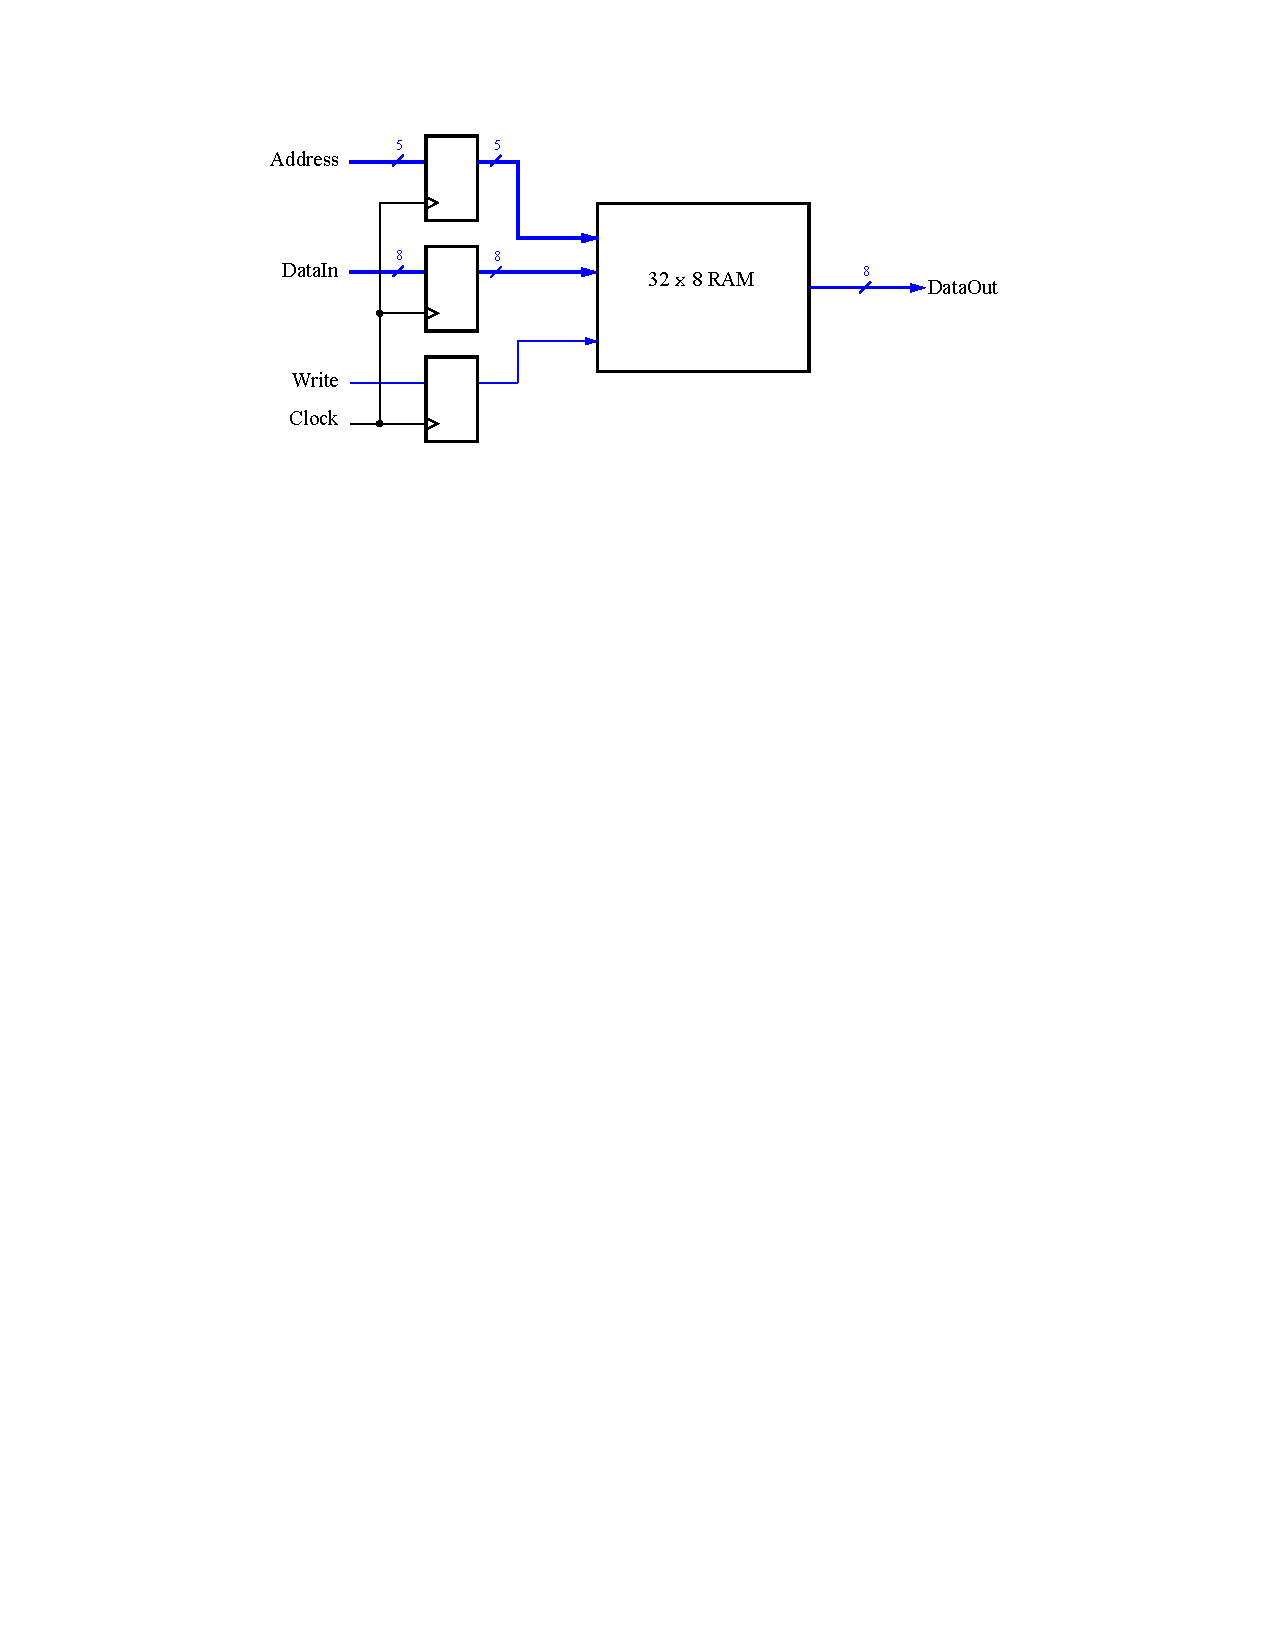
\includegraphics[]{figures/figure_RAM.pdf}
	\end{center}
	\caption{The 32 {\sf x} 8 RAM with address register.}
	\label{fig:fig_RAM}
\end{figure}

~\\
To place data into the memory, you need to specify {\it initial values}
that should be stored in the memory once your circuit has been programmed into the FPGA chip.
This can be done by initializing the memory using the contents of a {\it memory initialization 
file (MIF)}. The appropriate screen is illustrated in Figure~\ref{fig:fig7}. We have specified 
a file named {\it my\_array.mif}, which then has to be created in the folder that 
contains the Quartus project. An example of a memory initialization file is given in 
Figure~\ref{fig:fig_MIF}.  Set the contents of your {\it MIF} file such that it contains a
sorted collection of integers.

\begin{figure}[H]
	\begin{center}
		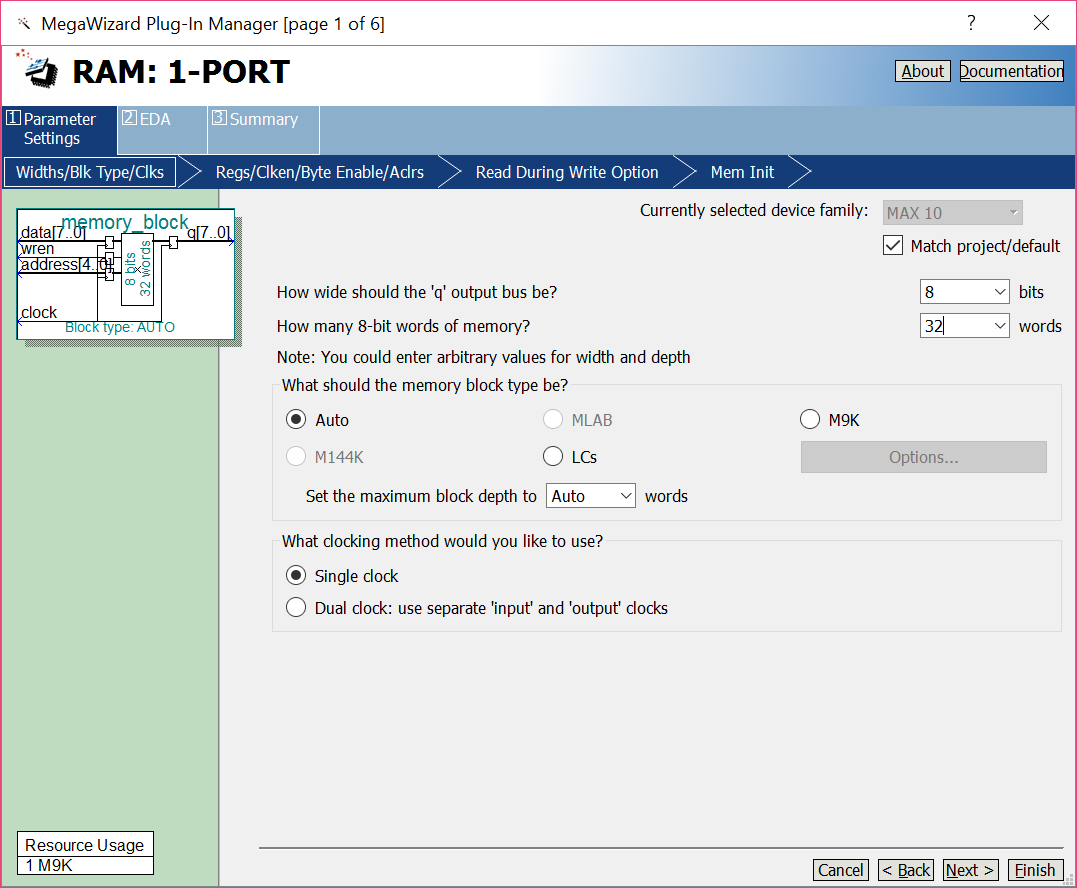
\includegraphics[scale=0.4]{figures/figure5.png}
	\end{center}
	\caption{{Specifying memory size.}}
	\label{fig:fig5}
\end{figure}

\begin{figure}[H]
	\begin{center}
		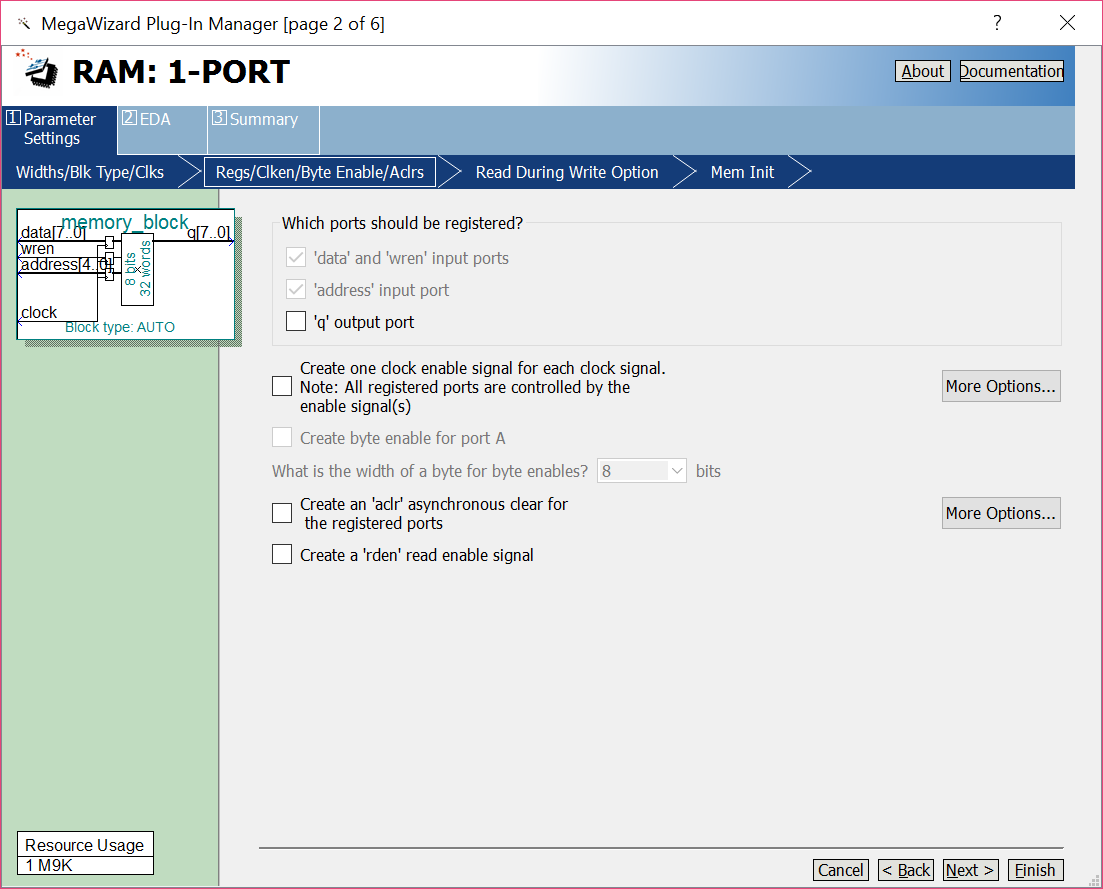
\includegraphics[scale=0.4]{figures/figure6.png}
	\end{center}
	\caption{Specifying which memory ports are registered.}
	\label{fig:fig6}
\end{figure}

\begin{figure}[H]
	\begin{center}
		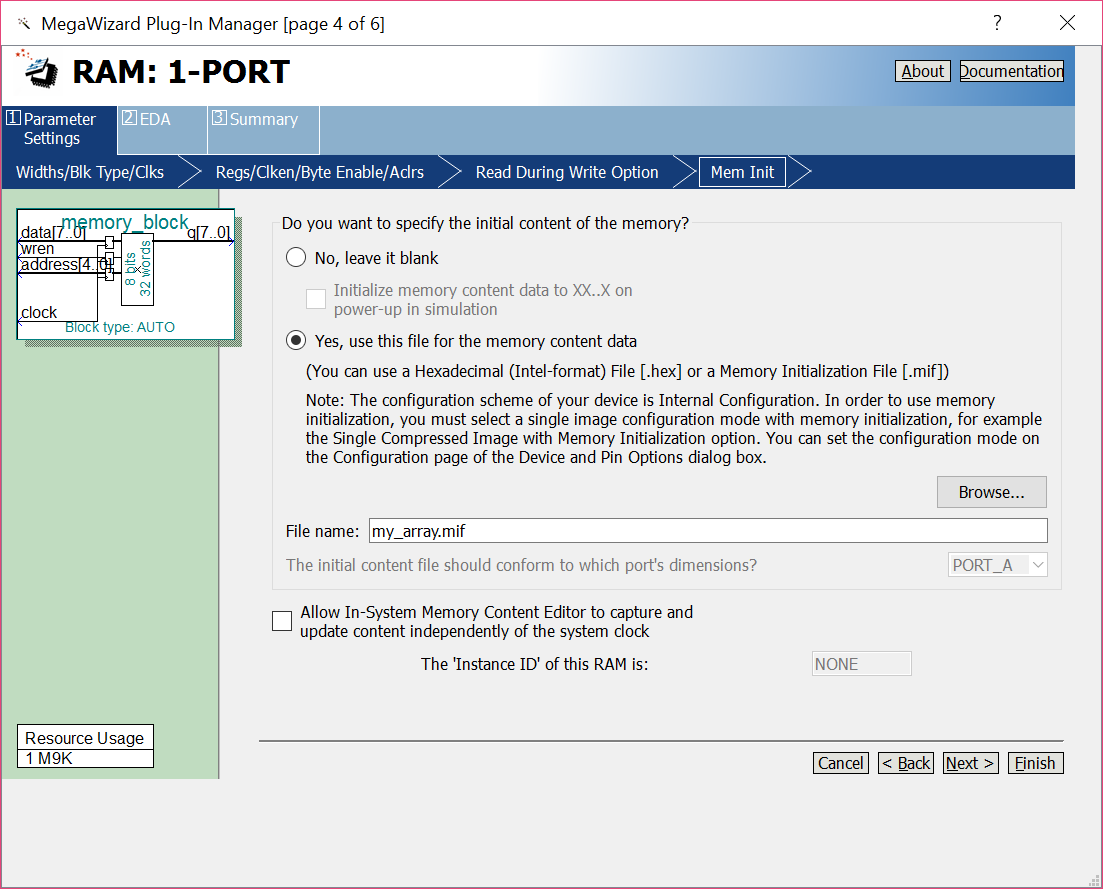
\includegraphics[scale=0.4]{figures/figure7.png}
	\end{center}
	\caption{Specifying a memory initialization file (MIF).}
	\label{fig:fig7}
\end{figure}

\begin{figure}[H]
\begin{center}
\begin{minipage}[t]{12.5 cm}
\begin{tabbing}
{\bf DEPTH} = 32;\\
{\bf WIDTH} = 8;\\
{\bf ADDRESS\_RADIX} = HEX;\\
{\bf DATA\_RADIX} = BIN;\\
{\bf CONTENT}\\
{\bf BEGIN}\\
\\
00	:	01;\\
01	:	02;\\
02	:	03\\
03	:	05;\\
04	:	06;\\
05	:	06;\\
06	:	07;\\
$\ldots$ (some lines not shown)\\
1E :	1F;\\
1F :	20;\\
\\
{\bf END};\\
\end{tabbing}
\end{minipage}
\end{center}
\caption{An example memory initialization file (MIF).}
\label{fig:fig_MIF}
\end{figure}

Your circuit should produce a 5-bit output {\it L}, which specifies the address in the memory 
where the number {\it A} is located. In addition, a signal
{\it Found} should be set high to indicate that the number {\it A} was found in the memory, 
and set low otherwise.

~\\
Perform the following steps:
\begin{enumerate}
\item Create an ASM chart for the binary search algorithm. Keep in mind that the memory
has registers on its input ports.  Assume that the array has a fixed size of 32 elements.
\item Implement the FSM and the datapath for your circuit.
\item Connect your FSM and datapath to the memory block as indicated in 
Figure~\ref{fig:binary_search_cct}.
\item Include in your project the necessary pin assignments to implement your circuit on
your DE-series board. Use switch {\it SW}$_{9}$ to drive the {\it Start} input, 
use {\it SW}$_{7{\ldots}0}$ to specify the value {\it A}, use 
{\it KEY}$_0$ for {\it Resetn}, and use the board's 50 MHz clock signal 
as the {\it Clock} input (be sure to synchronize the {\it Start} input to the clock). 
Display the address of the data $A$, if found, on 7-segment displays
{\it HEX}1 and {\it HEX}0, as a hexadecimal number.  Finally, use
{\it LEDR}$_{9}$ for the {\it Found} signal. 
\item Create a file called {\it my\_array.mif} and fill it with an ordered set of 32 
eight-bit integer numbers. 
\item Compile your design, and then download and test it.
\end{enumerate}


%%%%%%%%%%%%%%%%%%%%%%%%%%%%%%%%%%%%%%%%
%%% FPGAcademy Copyright Information %%%
%%%%%%%%%%%%%%%%%%%%%%%%%%%%%%%%%%%%%%%%

%Always put the copyright on a new page (clear page), with some vertical space from top
\clearpage
\vspace{1in}

\noindent

Copyright {\copyright} FPGAcademy.org. All rights reserved. FPGAcademy and the 
FPGAcademy logo are trademarks of FPGAcademy.org.  This document is provided 
"as is", without warranty of any kind, express or implied, including but not 
limited to the warranties of merchantability, fitness for a particular purpose 
and noninfringement. In no event shall the authors or copyright holders be 
liable for any claim, damages or other liability, whether in an action of 
contract, tort or otherwise, arising from, out of or in connection with the 
document or the use or other dealings in the document.
~\\
~\\
**Other names and brands may be claimed as the property of others.


\end{document}
